% 磁场中闭合电流的力矩
% 力矩|安培力|闭合回路

\pentry{磁矩\upref{MagMom}, 梯度\upref{Grad}}
\begin{figure}[ht]
\centering
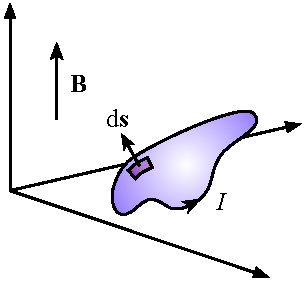
\includegraphics[width=5.5cm]{./figures/EBTorq_1.pdf}
\caption{闭合电流在磁场中所受的力矩} \label{EBTorq_fig1}
\end{figure}

如\autoref{EBTorq_fig1}, 在匀强磁场 $\bvec B$ 中, 一段闭合环路电流(忽略粗细)所受的力矩为
\begin{equation}\label{EBTorq_eq2}
\bvec \tau = \bvec \mu \cross \bvec B
\end{equation}
其中 $\bvec \mu$ 是\textbf{磁矩(megnetic moment)}, 等于电流 $I$ 乘以以这个环路为边界的任意曲面的面积矢量, 曲面法向量的方向通过右手定则\upref{RHRul}判断.
\begin{equation}
\bvec \mu = I \bvec A
\end{equation}
其中面积矢量 $\bvec A$ 的定义为(简单来说就是把\autoref{EBTorq_fig1} 中曲面上的所有小面积元求矢量和)
\begin{equation}
\bvec A = \oint \dd{\bvec s}
\end{equation}
一种简单的情况是, 若闭合环路在同一个平面上, 那么 $\bvec A$ 的模长就等于环路围成的面积.

更一般地, 若磁场为非匀强, 则力矩为
\begin{equation}\label{EBTorq_eq1}
\bvec \tau = I \int \dd{\bvec s}\cross\grad(\bvec B\vdot\bvec r)
\end{equation}

\subsection{推导}
\pentry{连续叉乘进行化简\upref{TriCro}, 斯托克斯定理\upref{Curl}}
如\autoref{EBTorq_fig1}, 线圈中有闭合电流 $I$, 以及任意磁场分布 $\bvec B(\bvec r)$, 现在求线圈所受力矩.我们可以把线圈划分为许多小段 $\dd{\bvec r}$,每小段的安培力产生的力矩为
\begin{equation}
\dd{\bvec \tau} = \bvec r\cross \dd{\bvec F} = \bvec r \cross (I \dd{\bvec r} \cross \bvec B)
\end{equation}
对连续叉乘进行化简\upref{TriCro} 得
\begin{equation}
\begin{aligned}
\dd{\bvec \tau} &=  \bvec r \cross (I\dd{\bvec r} \cross \bvec B) =  I (\bvec B \vdot \bvec r) \dd{\bvec r}  -  I\bvec B (\bvec r \vdot \dd{\bvec r})
\end{aligned}
\end{equation}
对 $\bvec r$ 沿闭合回路进行环积分得总力矩为
\begin{equation}
\begin{aligned}
\bvec \tau & = \int \dd{\bvec \tau} = I\oint (\bvec B\vdot\bvec r)\dd{\bvec r}  - I\bvec B\oint \bvec r \vdot \dd{\bvec r}
\end{aligned}
\end{equation}
其中
\begin{equation}
\oint \bvec r \vdot \dd{\bvec r}  = \oint r \uvec r \vdot \dd{\bvec r}  = \oint r \dd{r}  = \eval{\frac{r^2}{2}}_{r_0}^{r_0}  = 0 % 未完成: 这个符号有介绍吗?
\end{equation}
这是因为环积分的起点和终点到原点的距离都相同. 所以
\begin{equation}\ali{
\bvec \tau &= I \oint (\bvec B \vdot \bvec r) \dd{\bvec r} \\
&= \uvec x I \oint (\bvec B \vdot \bvec r)\uvec x \vdot \dd{\bvec r}  + \uvec y I \oint (\bvec B \vdot \bvec r)\uvec y \vdot \dd{\bvec r}  + \uvec zI \oint (\bvec B \vdot \bvec r)\uvec z \vdot \dd{\bvec r}
}\end{equation} 
对第一项进行分析,剩下两项类推即可. 由斯托克斯定理得
\begin{equation}
\begin{aligned} 
\uvec x I \oint (\bvec B \vdot \bvec r)\uvec x \vdot \dd{\bvec r}  &= \uvec x I \int \curl [ ( \bvec B \vdot \bvec r)\uvec x] \vdot \dd{\bvec s} \\
&= \uvec x I \int \grad (\bvec B \vdot \bvec r) \cross \uvec x \vdot \dd{\bvec s} \\
&= \uvec x I \int \dd{\bvec s}  \cross \grad (\bvec B \vdot \bvec r) \vdot \uvec x 
\end{aligned} 
\end{equation}
其中面积分在以环路为边界的任意曲面进行.对 $\uvec y$ 和 $\uvec z$ 项也同样处理, 得\autoref{EBTorq_eq1}. 在匀强电场的情况下, $\bvec B$ 是常矢量, $\grad (\bvec B \vdot \bvec r) = \bvec B$, 得\autoref{EBTorq_eq2}.
